\section{Basic}
    \subsection{vimrc}
        \lstinputlisting [language=bash] {Basic/vimrc}
    \subsection{int128}
        \lstinputlisting [language=bash] {Basic/int128.cpp}

\section{Flow}
    \subsection{Dinic}
        \lstinputlisting [language=c++] {Flow/Dinic.cpp}
    \subsection{MCMF}
        \lstinputlisting [language=c++] {Flow/MCMF.cpp}

\section{DataStructure}
    \subsection{SegmentTree}
        \lstinputlisting [language=c++] {DataStructure/SegmentTree.cpp}
    \subsection{KDTree}
        \lstinputlisting [language=c++] {DataStructure/KDTree.cpp}
    \subsection{BIT}
        \lstinputlisting [language=c++] {DataStructure/BIT.cpp}
    \subsection{DisjointSet}
        \lstinputlisting [language=c++] {DataStructure/djs.cpp}
    \subsection{HeavyLightDecomposition}
        \lstinputlisting [language=c++] {DataStructure/HeavyLightDecomposition.cpp}
    \subsection{LCA}
        \lstinputlisting [language=c++] {DataStructure/LCA.cpp}
    \subsection{MO}
        \lstinputlisting [language=c++] {DataStructure/MO.cpp}
    \subsection{PartitionTree}
        \lstinputlisting [language=c++] {DataStructure/PartitionTree.cpp}
    \subsection{PersistentSegmentTree}
        \lstinputlisting [language=c++] {DataStructure/PersistentSegmentTree.cpp}
    \subsection{PersistentTreap}
        \lstinputlisting [language=c++] {DataStructure/PersistentTreap.cpp}
    \subsection{SparseTable}
        \lstinputlisting [language=c++] {DataStructure/SparseTable.cpp}
    \subsection{pbds\_heap}
        \lstinputlisting [language=c++] {DataStructure/pbds_heap.cpp}
    \subsection{pbds\_tree}
        \lstinputlisting [language=c++] {DataStructure/pbds_tree.cpp}
    \subsection{unordered\_map}
        \lstinputlisting [language=c++] {DataStructure/unordered_map.cpp}


\section{Geometry}
    \subsection{ClosestPair}
        \lstinputlisting [language=c++] {Geometry/ClosestPair.cpp}
    \subsection{Geometry}
        \lstinputlisting [language=c++] {Geometry/Geometry.cpp}
    \subsection{MinCoverCircle}
        \lstinputlisting [language=c++] {Geometry/MinCoverCircle.cpp}

\section{DP}
    \subsection{KnapsackLimit}
        \lstinputlisting [language=c++] {DP/KnapsackLimit.cpp}

\section{Graph}
    \subsection{BCC}
        \lstinputlisting [language=c++] {Graph/BCC.cpp}
    \subsection{Blossom}
        \lstinputlisting [language=c++] {Graph/Blossom.cpp}
    \subsection{CutBridge}
        \lstinputlisting [language=c++] {Graph/CutBridge.cpp}
    \subsection{Dijkstra}
        \lstinputlisting [language=c++] {Graph/Dijkstra.cpp}
    \subsection{MaximumClique}
        \lstinputlisting [language=c++] {Graph/MaximumClique.cpp}
    \subsection{MinMeanCycle}
        \lstinputlisting [language=c++] {Graph/MMC.cpp}
    \subsection{SCC}
        \lstinputlisting [language=c++] {Graph/SCC.cpp}
    \subsection{KM}
        \lstinputlisting [language=c++] {Graph/KM.cpp}
    \subsection{GridMST}
        \lstinputlisting [language=c++] {Graph/GridMST.cpp}

\section{Math}
    \subsection{bigN}
        \lstinputlisting [language=c++] {Math/bigN.cpp}
    \subsection{BSGS}
        \lstinputlisting [language=c++] {Math/BSGS.cpp}
    \subsection{CRT}
        \lstinputlisting [language=c++] {Math/CRT.cpp}
    \subsection{ExtgcdModInv}
        \lstinputlisting [language=c++] {Math/ExtgcdModInv.cpp}
    \subsection{FFT}
        \lstinputlisting [language=c++] {Math/FFT.cpp}
    \subsection{Matrix}
        \lstinputlisting [language=c++] {Math/Matrix.cpp}
    \subsection{Mobius}
        \lstinputlisting [language=c++] {Math/Mobius.cpp}
    \subsection{PHITable}
        \lstinputlisting [language=c++] {Math/PHITable.cpp}
    \subsection{MillerRabin}
        \lstinputlisting [language=c++] {Math/MillerRabin.cpp}
    \subsection{PrimativeRoot}
        \lstinputlisting [language=c++] {Math/primativeRoot.cpp}
    \subsection{Simplex}
        \lstinputlisting [language=c++] {Math/simplex.cpp}
    \subsection{PollardRho}
        \lstinputlisting [language=c++] {Math/PollardRho.cpp}

\section{String}
    \subsection{ACAutomaton}
        \lstinputlisting [language=c++] {String/ACAutomaton.cpp}
    \subsection{Eertree}
        \lstinputlisting [language=c++] {String/Eertree.cpp}
    \subsection{KMP}
        \lstinputlisting [language=c++] {String/KMP.cpp}
    \subsection{minRotation}
        \lstinputlisting [language=c++] {String/minRotation.cpp}
    \subsection{SA}
        \lstinputlisting [language=c++] {String/SA.cpp}
    \subsection{SAM}
        \lstinputlisting [language=c++] {String/SAM.cpp}
    \subsection{Z}
        \lstinputlisting [language=c++] {String/Z.cpp}
    \subsection{BWT}
        \lstinputlisting [language=c++] {String/bwt.cpp}
    \subsection{IBWT}
        \lstinputlisting [language=c++] {String/ibwt.cpp}

\section{Other}
    \subsection{Python}
        \lstinputlisting [language=python] {Other/python_sheet.py}
    \subsection{GNU\_bitwise}
        \lstinputlisting [language=c++] {Other/GNU_bitwise.cpp}
    \subsection{Count\_Spanning\_Tree}
        \lstinputlisting [language=c++] {Other/count_spanning_tree.cpp}
    \subsection{Count\_Digit}
        \lstinputlisting [language=c++] {Other/CountDigit.cpp}

\onecolumn
\centering
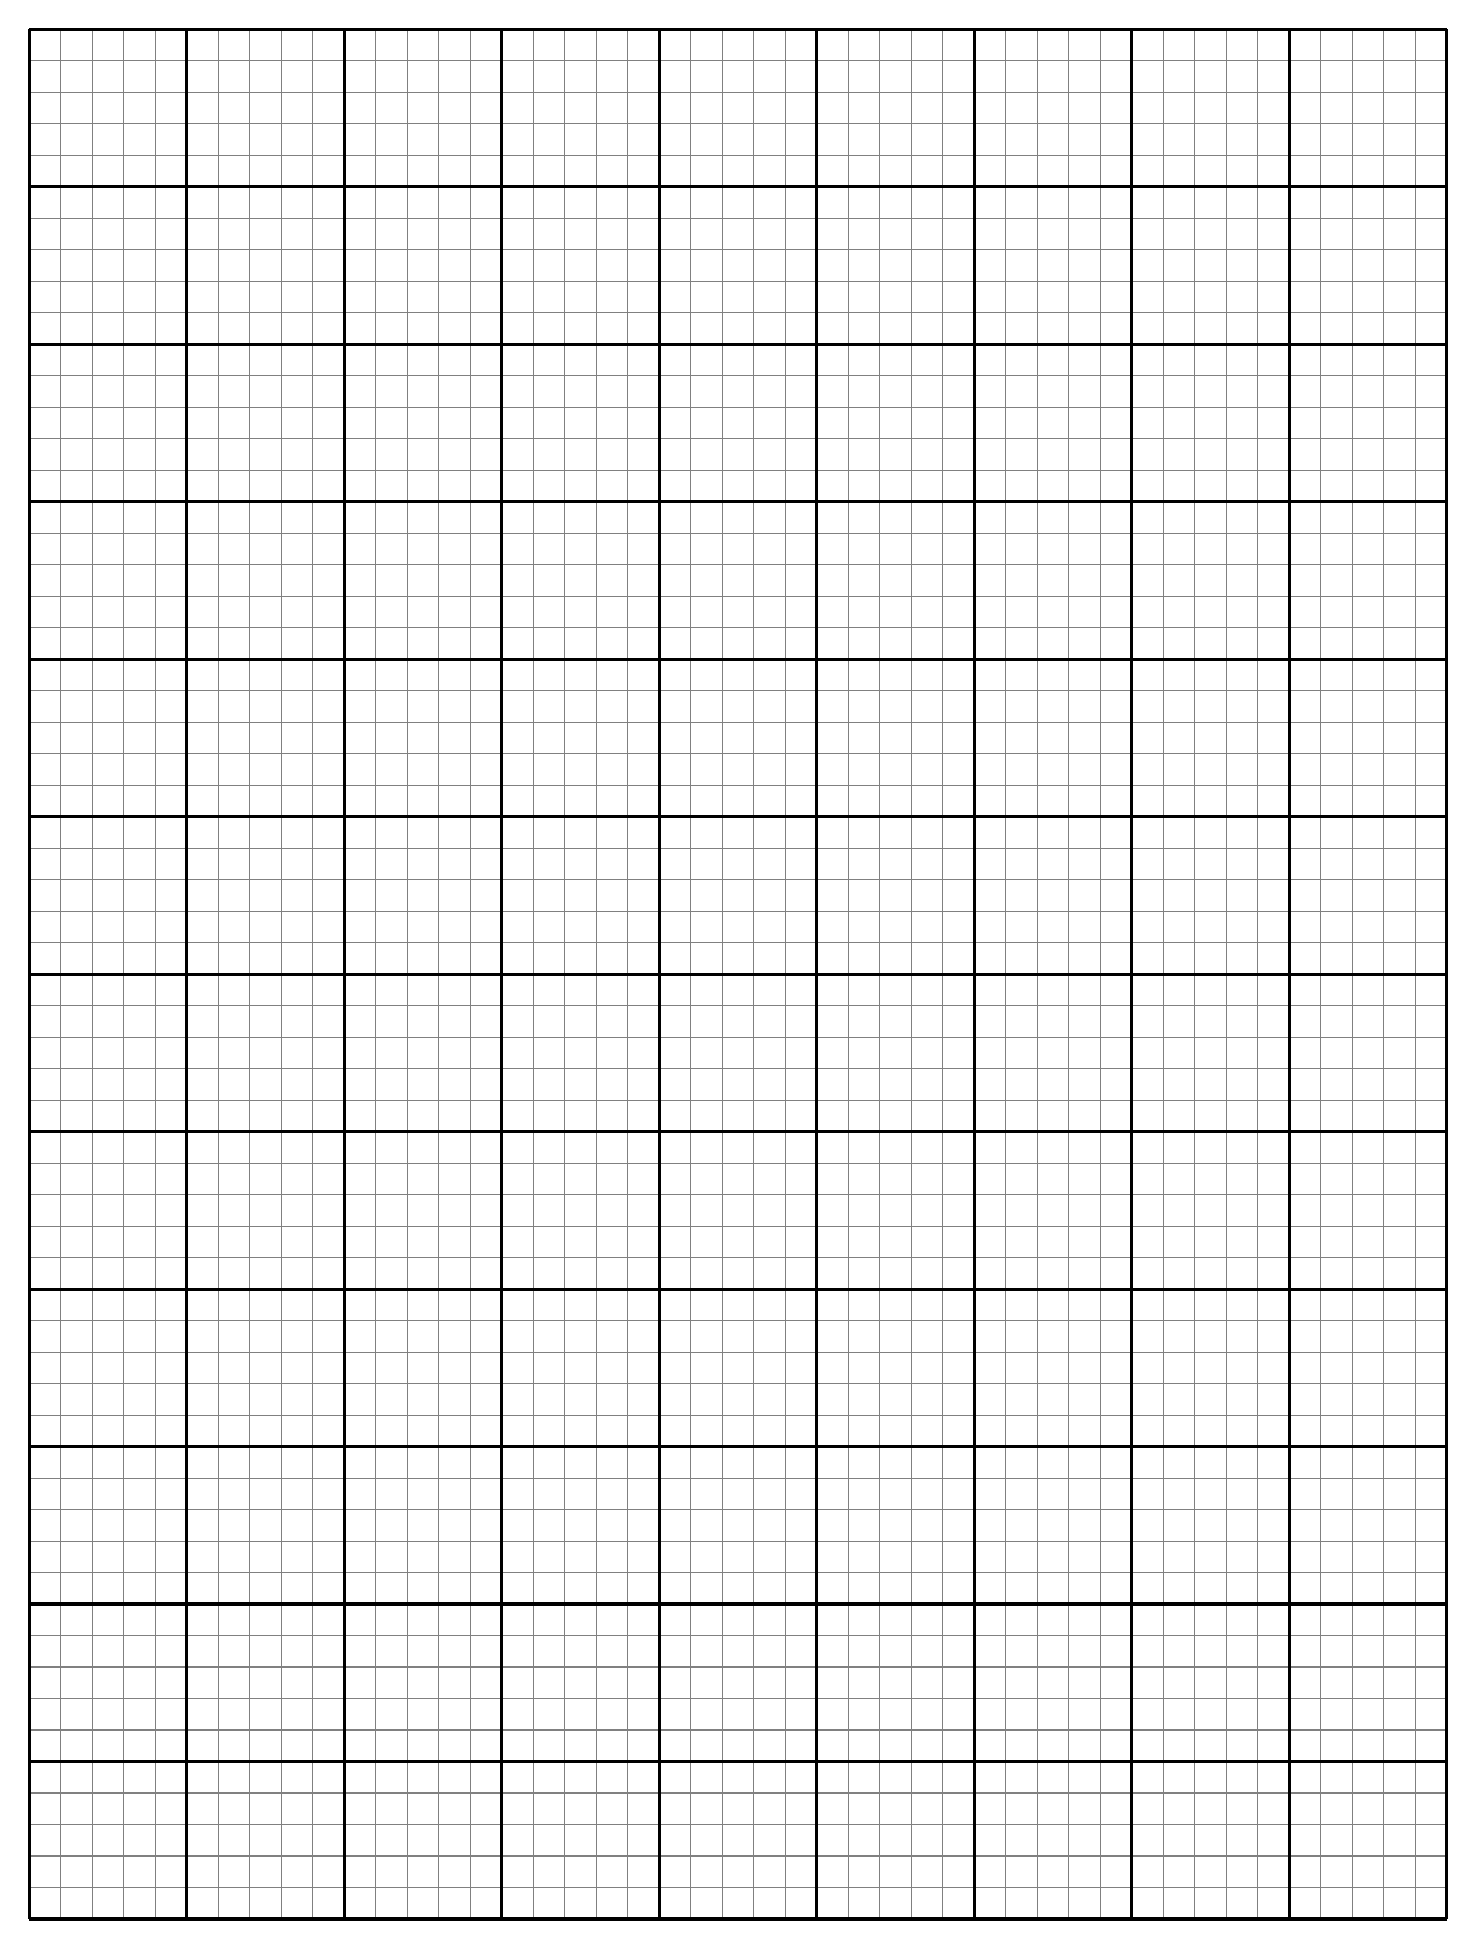
\begin{tikzpicture}[every node/.style={minimum size=1cm-\pgflinewidth, outer sep=10pt}, scale=2]
    \draw[step=0.2cm,color=gray] (0,0) grid (9,12);
    \draw[step=1cm,color=black,line width=0.4mm] (0,0) grid (9,12);
\end{tikzpicture}
